\documentclass[12pt,a4paper]{exam}
\usepackage[utf8]{inputenc}
\usepackage[T1]{fontenc}
\usepackage{amsmath}
\usepackage{amsfonts}
%\usepackage{amssymb}
\usepackage{graphicx}
\usepackage{geometry}
\usepackage{enumitem}

\geometry{a4paper, margin=2cm}

\usepackage{cprotect}

\usepackage{xcolor}
\definecolor{maroon}{cmyk}{0, 0.87, 0.68, 0.32}
\definecolor{halfgray}{gray}{0.55}
\definecolor{ipython-frame}{RGB}{207, 207, 207}
\definecolor{ipython-bg}{RGB}{247, 247, 247}
\definecolor{ipython-red}{RGB}{186, 33, 33}
\definecolor{ipython-green}{RGB}{0, 128, 0}
\definecolor{ipython-cyan}{RGB}{64, 128, 128}
\definecolor{ipython-purple}{RGB}{170, 34, 255}
\usepackage{listings}
\lstdefinelanguage{iPython}{
	morekeywords={access,and,del,except,exec,in,is,lambda,not,or,raise},
	morekeywords=[2]{for,print,abs,all,any,basestring,bin,bool,bytearray,callable,chr,classmethod,cmp,compile,complex,delattr,dict,dir,divmod,enumerate,eval,execfile,file,filter,float,format,frozenset,getattr,globals,hasattr,hash,help,hex,id,input,int,isinstance,issubclass,iter,len,list,locals,long,map,max,memoryview,min,next,object,oct,open,ord,pow,property,range,reduce,reload,repr,reversed,round,set,setattr,slice,sorted,staticmethod,str,sum,super,tuple,type,unichr,unicode,vars,xrange,zip,apply,buffer,coerce,intern,elif,else,if,continue,break,while,class,def,return,try,except,import,finally,try,except,from,global,pass, True, False},
	sensitive=true,
	morecomment=[l]\#,%
	morestring=[b]',%
	morestring=[b]",%
	moredelim=**[is][\color{black}]{@@}{@@},
	identifierstyle=\color{black}\footnotesize\ttfamily,
	commentstyle=\color{ipython-cyan}\footnotesize\itshape\ttfamily,
	stringstyle=\color{ipython-red}\footnotesize\ttfamily,
	keepspaces=true,
	showspaces=false,
	showstringspaces=false,
	rulecolor=\color{ipython-frame},
	frame=single,
	frameround={t}{t}{t}{t},
	backgroundcolor=\color{ipython-bg},
	basicstyle=\footnotesize\ttfamily,
	keywordstyle=[2]\color{ipython-green}\bfseries\footnotesize\ttfamily, 
	keywordstyle=\color{ipython-purple}\bfseries\footnotesize\ttfamily
}

\lstdefinelanguage{iOutput} {
	sensitive=true,
	identifierstyle=\color{black}\small\ttfamily,
	stringstyle=\color{ipython-red}\small\ttfamily,
	keepspaces=true,
	showspaces=false,
	showstringspaces=false,
	rulecolor=\color{ipython-frame},
	basicstyle=\small\ttfamily,
}

\lstnewenvironment{ipython}[1][]{\lstset{language=iPython,mathescape=true,escapeinside={*@}{@*}}%
}{%
}

\lstnewenvironment{ioutput}[1][]{\lstset{language=iOutput,mathescape=true,escapeinside={*@}{@*}}%
}{%
}

\title{Financial Market Course 22/23\\ Exam}
\author{Prof. Simone Freschi, Prof. Matteo Sani}
\date{$12^{\mathrm{st}}$ July 2023}

\printanswers
%\noprintanswers
\begin{document}
\maketitle

\begin{center}
\fbox{\fbox{\parbox{5.5in}{\centering
Answer the questions in the spaces provided. If you run out of room for an answer, continue on the page back.}}}
\end{center}

\begin{center}
\vspace{5mm}
\makebox[0.75\textwidth]{Student's name:\enspace\hrulefill}
\end{center}

\section*{Questions}
\vspace{.5cm}
\begin{questions}
\question
Monte Carlo techniques are quite useful in order to approximate expectations
\begin{equation*}
\mathbb{E}[f(X)] = \frac{1}{n}\sum_{i=1}^n f(x_i)
\end{equation*} 
by sampling $n$ times from the probability density of $X$.
Previous approximation works in the limit of a large number of events and under the assumption that $\{x_1, x_2\ldots,x_n\}$ are \emph{independent and identically distributed random variables}.
Write a dummy \texttt{python} implementation of a Monte Carlo simulation explaining the details of the used strategy.
\makeemptybox{5cm}
\begin{solution}
\begin{ipython}
import numpy as np
from scipy.stats import norm

N = 10000
s = 0
for i in range(N):
    np.random.seed(i)
    x = np.random.uniform(-10, 10)
    s += x*norm.pdf(x)

print (s/N)
\end{ipython}
\begin{ioutput}
-0.0014062275161523389
\end{ioutput}
\end{solution}

%%%%%%%%%%%%%%%%%%%%%%%%%%%%%%%%%%%%%%%%%%%%%%%%%%%%%%%%%%%%%
\question
Consider a portfolio whose efficient frontier is described by the following curve and assume that a risk-free investment yields $r_f = 10\%$.
\begin{center}
  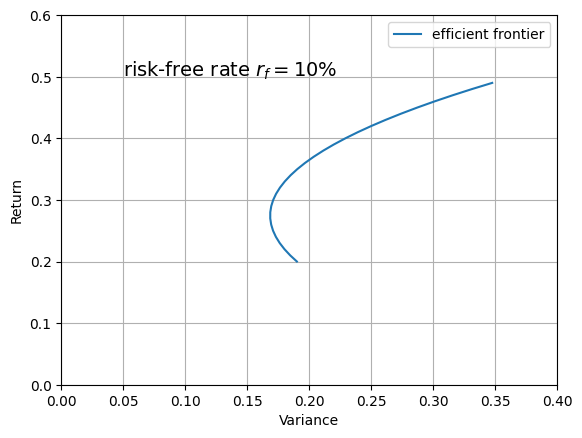
\includegraphics[width=0.7\linewidth]{efficient_frontier}
\end{center}
Using the plot determine the numerical value of the Sharpe ratio corresponding to the asset allocation of the portfolio maximizing it.
\fillwithlines{3cm}
\begin{solution}
In the Variance-Return plane the Sharpe portfolio can be identified by the tangent point between the efficient frontier and the CAL (the line passing through $(0.0, r_f)$. From the given plot this point lies approximately at $(0.2, 0.37)$ so
\begin{equation*}
  SR = \frac{r_P - r_f}{\sigma_P} = \frac{0.37-0.1}{0.2} \approx 1.35
\end{equation*}
\end{solution}

%%%%%%%%%%%%%%%%%%%%%%%%%%%%%%%%%%%%%%%%%%%
\question
Write a \texttt{python} function that computes a coupon-bearing bond price given: notional, coupon, risk-free rate, time-to-maturity, and tenor.
\textbf{Note:} for simplicity consider a flat risk-free rate.
\fillwithlines{3cm}
\begin{solution}
  \begin{ipython}
def bond_price(N, C, r, ttm, tau):
    price = 0
    for t in range(1, ttm+1):
        price += N*tau*C/(1+r)**t
    price += N/(1+r)**t
    return price    
    \end{ipython}
\end{solution}

%%%%%%%%%%%%%%%%%%%%%%%%%%%%%%%%%%%%%%%%%%%
\question
What is the output of the following \texttt{python} code

\begin{ipython}
mylist = [1,2,3,4,5]*3
\end{ipython}
\fillwithlines{3cm}
\begin{solution}
Contrary to what one may expect the output will be
\begin{ioutput}
[1,2,3,4,5,1,2,3,4,5,1,2,3,4,5]
\end{ioutput}
and NOT
\begin{ioutput}
[3,6,9,12,15]
\end{ioutput}
\end{solution}
%%%%%%%%%%%%%%%%%%%%%%%%%%%%%%%%%%%%%%%%%%%
\question
What is the output of the following \texttt{python} code

\begin{ipython}
for x in range(0.5, 5.5, 0.5):
    print(x)
\end{ipython}
\fillwithlines{3cm}
\begin{solution}
The program will result in a
\begin{ioutput}
TypeError: 'float' object cannot be interpreted as an integer
\end{ioutput}
since the built-in function \texttt{range} accepts only integer arguments. To use floats must move to \texttt{numpy.arange} which is more general.
\end{solution}

\end{questions}
\end{document}
